\documentclass[titlepage=true,11pt,a4paper]{scrartcl}

\usepackage[ngerman]{babel}
\usepackage[utf8]{inputenc}
\usepackage{lmodern}
\usepackage{units}
\usepackage{graphicx}
\usepackage{float}
\usepackage{pdfpages}
\usepackage{tikz}
\usetikzlibrary{shapes.geometric, arrows}
\usepackage{multirow}
\usepackage{lscape}
\usepackage{amsmath, amsfonts, amssymb, mathtools, empheq}
\usepackage{listings}
\usepackage{color}

\renewcommand\lstlistlistingname{Quellcode}

\begin{document}
	\vfill
	\subject{Dokumentation}
	\title{Roboter-Fangen}
	\subtitle{Maschinenbauinformatik 3. \& 5. Semester}
	\author{Michael Mertens, Jonah Vennemann, Sven Stegemann, Eugen Zwetzich}
	\date{\today}
	\maketitle
	\newpage
	\setcounter{page}{1}
	\tableofcontents
	\newpage
	\listoffigures
	\lstlistoflistings
	\newpage
	
	\section{Vorgaben}
\subsection{Projektbeschreibung}
Bei dem Projekt "`Roboter-Fangen"' für das Modul IT-Projektmanagement besteht unsere Aufgabe als eines von zwei Teams in der Programmierung einer Steuerungssoftware für das Fischertechnik ROBOTICS TXT Discovery Set.

Das Gemeinziel ist ein lauffähiges Fangen-Spiel zu erstellen bei dem vier Roboter pro Team von der jeweiligen Software gesteuert werden.

Dabei werden die Positionsdaten aller Roboter von einem Schiedsrichter-Server mit Hilfe einer Kamera berechnet und an die Steuerungssoftware der beiden Teams geschickt.
Hauptbestandteile der Steuerungssoftware:
\begin{itemize}
	\item Benutzeroberfläche:
	\begin{itemize}
		\item Kamerabilder
		\item Eingabefelder zum Verbinden
		\item zusätzliche Informationen
	\end{itemize}
	\item Positionsdatenverarbeitung über eine Vektorklasse:
	\begin{itemize}
		\item Attribute: x,y als Typ Double
		\item Methoden: Addieren, Subtrahieren, Skalar multiplizieren, Winkel berechnen
	\end{itemize}
	\item Elemente der KI:
	\begin{itemize}
		\item Fangen
		\item Fliehen
		\item Ausweichen
		\item im Feld bleiben
		\item Rausfahren nachdem Gefangenwerden\\
	\end{itemize}
\end{itemize}
Neben der Programmierung gehören dabei auch die Planung, die Dokumentation des Codes sowie die Darstellung des Projekts dazu.
\begin{itemize}
	\item Quelltextkommentare
	\item Präsentation
	\item Zeiterfassung
	\item Betriebsanleitung
	\item Spielregeln
\end{itemize}
	\subsection{Spielablauf}
\begin{center}
	\includegraphics[width=0.8\textwidth]{Bilder/Spielfeld_2.pdf}
\end{center}
Es werden pro Gruppe 4 Roboter auf dem Spielfeld an ihre Startpositionen platziert.
Die Größe des Spielfeldes ist festgelegt.

Alle Roboter, von beiden Teams, verbinden sich mit dem Server und übergeben diesem, dass Sie bereit sind.
Sobald der Server das Startsignal gibt, fahren die Roboter mit einer Geschwindigkeit die $\frac{3}{4}$ der
vollen Geschwindigkeit entspricht los.

Dann versuchen sich die Roboter, der beiden Teams, gegenseitig zu fangen. Dazu muss einer der beiden Taster, welche am hinteren Ende des Roboters angebracht sind, betätigt werden.

Befindet sich ein gegnerischer Roboter im Abstand X vor einem anderer Roboter, so wird die maximale Geschwindigkeit des hinteren Roboters freigeschaltet.

Wenn ein Roboter gefangen wurde, sendet dieser ein Signal an den Server und wird von diesem auf nicht Aktiv gesetzt.
Ist ein Roboter nicht Aktiv, so fährt dieser aus dem Spielfeld und verbleibt dort eine gewisse Zeit, bis er in's Spiel zurück kehrt.\\
\newline
Folgende Regeln wurden getroffen:
\begin{itemize}
	\item Ein Roboter darf erst losfahren, wenn der Server das Startsignal gegeben hat
	\item Ein Roboter darf sich nicht auf der Stelle drehen
	\item Ein Roboter darf nicht mit dem Rücken zur Wand stehen, da es so nicht möglich ist diesen zu fangen 
	\item Erst ab einem Abstand X, darf die volle Geschwindigkeit zur Verfügung stehen
\end{itemize}
	\section{Gantt-Diagramm}
Ein Gantt-Diagramm oder auch Balkenplan ist ein nach dem Unternehmensberater Henry L. Gantt benanntes Instrument des Projektmanagements, das die zeitliche Abfolge von Aktivitäten grafisch in Form von Balken auf einer Zeitachse darstellt.

In der Abbildung 1 sieht man die einzelnen Aktivitäten, die wir für unser Projekt Roboter-Fangen eingeplant haben.
Außerdem sieht

Einige Aktivitäten haben wir in Gruppen eingeteilt, um:
\begin{itemize}
	\item Planung
	\item Programmierung - Teil 1
	\item Programmierung - Teil 2
	\item Dokumentation
\end{itemize}

\begin{center}
	\begin{figure}[H]
		\includegraphics[scale=0.5]{Bilder/GanttDiagramm_[Page1].pdf}
		\includegraphics[scale=0.5]{Bilder/GanttDiagramm_[Page2].pdf}
		\caption{Gantt-Diagramm}
	\end{figure}
\end{center}

	\section{Aufwandsschätzung}
Um den Aufwand unseres IT-Projektes abschätzen zu können, haben wir die Methode Function-Point benutzt.

Das Function-Point-Verfahren(auch -Analys oder -Methode, kurz: FPA) dient der Bewertung des fachlich-funktionalen Umfangs eines Informationstechnischen Systems.\\
\newline
Die Durchführung des Verfahrens verläuft in 5 Schritten:
\begin{enumerate}
	\item Analyse der Komponenten und Kategorisierung ihrer Funktionalitäten
	\item Bewertung der verschiedenen Funktionskategorien
	\item Einbeziehung besonderer Einflussfaktoren
	\item Ermittlung der sog. Total Function Points(TFP)
	\item Ableitung des zu erwartenden Entwicklungsaufwandes
\end{enumerate}
\vspace{0.2cm}
\paragraph{1. Schritt}
\begin{itemize}
	\item Eingabedaten
	\begin{itemize}
		\item GUI
		\item Programmstart
	\end{itemize}
	\item Ausgabedaten
	\begin{itemize}
		\item Ereignisprotokolldatei
		\item Kamerabild
		\item Steuerbefehle senden
	\end{itemize}
	\item projektbez. Datenbestände
	\begin{itemize}
		\item Fahrtrichtung
		\item Fangen
		\item Fliehen
		\item Ausweichen
		\item Im Feld bleiben
		\item Rausfahren nach dem Fangen
		\item Vektorberechnung
	\end{itemize}
	\item externe Datenbestände
	\begin{itemize}
		\item Positionsdaten
		\item Mitteilung gefangen
		\item Roboter aktiv?
	\end{itemize}
\end{itemize}

\newpage
\begin{landscape}
	\paragraph{2. Schritt}
	\begin{center}
		\begin{tabular}{|l|ccc|ccc|ccc|}
			\hline
			\multirow{2}{*}{Funktionskategorie} & \multicolumn{3}{c|}{Anzahl der Funktionen} & \multicolumn{3}{c|}{Faktoren der Funktionen} & \multicolumn{3}{c|}{Funktionspunkte}\\
			& Einfach & Mittel & Komplex & Einfach & Mittel & Komplex & Einfach & Mittel & Komplex\\
			\hline
			Eingabedaten & 1 & 1 & 0 & 3 & 4 & 6 & 3 & 4 & 0\\
			Ausgabedaten & 1 & 2 & 0 & 4 & 5 & 7 & 4 & 10 & 0\\
			Projektbez. Datenbestände & 1 & 3 & 3 & 7 & 10 & 15 & 7 & 30 & 45\\
			Externe Datenbestände & 3 & 0 & 0 & 5 & 7 & 10 & 15 & 0 & 0\\
			\hline
			\multicolumn{10}{c}{}\\
			\cline{8-10}
			\multicolumn{7}{c}{} & \multicolumn{2}{|l|}{{\bf Summe S$1$:}} & {\bf $118$}\\
			\cline{8-10}			
		\end{tabular}
	\end{center}
	\vspace{0.2cm}
	\begin{minipage}{0.7\textwidth}
		\paragraph{3. Schritt}
		\begin{center}
			\begin{tabular}{|c|l|c|}
				\hline
				Nr & Einflussfaktoren & Gewichte\\
				\hline
				1 & Schwierigkeit und Komplexität der Rechenoperatoren (Faktor 2) & 2\\
				2 & Schwierigkeit und Komplexität der Ablauflogik & 5\\
				3 & Umfang der Ausnahmeregelung (Faktor 2) & 6\\
				4 & Verflechtungen mit anderen IT-Systemen & 3\\
				5 & dezentrale Verarbeitung und Datenhaltung & 0\\
				6 & erforderliche Maßnahmen der IT Sicherheit & 0\\
				7 & angestrebte Rechengeschwindigkeit & 1\\
				8 & Konvertierung der Datenbeständen & 0\\
				9 & Benutzer- und Änderungsfreundlichkeit & 1\\
				10 & Wiederverwendbarkeit von Komponenten (bspw. Klassen) & 1\\
				\hline
				\multicolumn{3}{c}{}\\
				\cline{2-3}
			    \multicolumn{1}{c}{} & \multicolumn{1}{|l|}{{\bf Summe S$2$:}} & $19$\\
				\cline{2-3} 
			\end{tabular}
		\end{center}
	\end{minipage}
\end{landscape}

\paragraph{4. Schritt}
\begin{align*}
	\text{TFP} &= \text{S}1 \cdot \text{S}3\\
			   &= \text{S}1 \cdot \left(0{,}7 + \frac{\text{S}2}{100}\right)\\
			   &= 118 \cdot \left( 0{,}7 + \frac{19}{100}\right)\\
	\text{TFP} &= 105{,}02\\
\end{align*}
\paragraph{5. Schritt}
\[\text{PM\footnotemark} = 0{,}08 \cdot \text{TFP}-7 \leq 1000\text{TFP} > \text{PM} = 0{,}08 \cdot \text{TFP}-108\]
\begin{align*}
	\text{PM} &= 0{,}08 \cdot \text{TFP} - 7 \\
			  &= 0{,}08 \cdot 105{,}02 -7\\
	\text{PM} &= 1{,}4016\\
	\\
	\text{PM} &= 672{,}77 \text{h}\\
	\\
	\text{3 Personen} &= 224{,}256\text{h pro Person}\\
	\text{4 Personen} &= 168{,}192\text{h pro Person}\\
\end{align*}\footnotetext{Personenmonate(PM) = 20 Arbeitstage}

$\Rightarrow$ Bei einem 4 starken Team benötigen wir ca. 170h pro Person.

	\section{GitHub}
GitHub ist ein webbasierter Online-Dienst, für die Versionsverwaltungssoftware Git.

Diesen Online-Dienst haben wir dafür benötigt, um von verschiedenen Standtorten und mit verschiedenen Mitarbeitern an dem Projekt arbeiten zu können.

Außerdem kann man sich anzeigen, welcher Mitarbeiter, wie lange an dem Projekt gearbeitet hat.
\begin{center}
	\includegraphics[width=1\textwidth]{Bilder/Github.pdf}
	\captionof{figure}{GitHub}
	\includegraphics[width=1\textwidth]{Bilder/GitHub_Mitarbeiter_Dauer.pdf}
	\captionof{figure}{GitHub Mitarbeiterzeit}
\end{center}
	
	\subsection{ZenHub}
ZenHub ist ein Projektmanagement Addon für GitHub.

In diesem ist es möglich
	\input{Inhalt/Bedienung.tex}
	\section{Programmierung}
\subsection{Programmablaufplan}
\vspace{1cm}
\begin{center}
	\tikzstyle{startstop} = [rectangle, rounded corners, minimum width=3cm, minimum height=1cm,text centered, draw=black, fill=red!30]
	\tikzstyle{io} = [trapezium, trapezium left angle=70, trapezium right angle=110, minimum width=3cm, minimum height=1cm, text centered, draw=black, fill=blue!30]
	\tikzstyle{process} = [rectangle, minimum width=3cm, minimum height=1cm, text centered, text width=3cm, draw=black, fill=orange!30]
	\tikzstyle{decision} = [diamond, minimum width=1cm, minimum height=1cm, text centered, text width=3cm, draw=black, fill=green!30]
	\tikzstyle{arrow} = [thick,->,>=stealth]
	\begin{tikzpicture}[node distance=2cm]
		\node (start) [startstop] {Start};
		\node (pro1) [process,below of=start] {Vordefinierter Anfangsweg};
		\node (in1) [io,below of=pro1] {Eingabedaten verarbeiten};
		\node (dec1) [decision,below of=in1,yshift=-1cm] {Roboter aktiv?};
		\node (dec2) [decision,below of=dec1,xshift=3.5cm,yshift=-2cm] {Priorität festlegen};
		\node (pro2) [process,below of=dec1,xshift=-4cm,yshift=-2cm] {Herausfahrvektor berechnen};
		\node (pro3) [process,below of=dec2,xshift=-4cm,yshift=-1.5cm] {Verfolgungsvektor berechnen};
		\node (pro4) [process,below of=dec2,xshift=4cm,yshift=-1.5cm] {Fliehvektor berechnen};
		\node (pro5) [process,below of=pro3,xshift=4cm,yshift=-1cm] {Vektor anpassen};
		\node (in2) [io,below of=pro5] {Befehle senden};
		
		\draw [arrow] (start) -- (pro1);
		\draw [arrow] (pro1) -- (in1);
		\draw [arrow] (in1) -- (dec1);
		\draw [arrow] (dec1) -| node[anchor=south] {ja} (dec2);
		\draw [arrow] (dec1) -| node[anchor=south] {nein} (pro2);
		\draw [arrow] (dec2) -| node[anchor=south] {fangen} (pro3);
		\draw [arrow] (dec2) -| node[anchor=south] {fliehen} (pro4);
		\draw [arrow] (pro2) |- (pro5);
		\draw [arrow] (pro3) -| (pro5);
		\draw [arrow] (pro4) -| (pro5);
		\draw [arrow] (pro5) -- (in2);
		\draw [arrow] (in2) -| (10.5, -8) |- (0,-3);
	\end{tikzpicture}
\end{center}
\newpage
\subsection{Benutzeroberfläche}

\subsection{Klassen}
Für die Berechnungen und Logik haben wir eigene Klassen geschrieben.\\
\newline
Diese unterteilen sich in:
\begin{itemize}
	\item mVektor
	\item mTKI
	\item mKonstanten
	\item mRoboterDaten
\end{itemize}

\subsubsection{mVektor}
Die Klasse mVektor besteht aus dem Record TVektor.

Dieser hat folgende Funktionen, überladende Operatoren und Variablen:
\begin{itemize}
	\item Funktionen
	\begin{description}
		\item[Winkel(überladen)] gibt den Winkel des Vektors, bezogen auf die X-Achse, zurück
		\item[Winkel(überladen)] gibt den Winkel zwischen zwei Vektoren zurück
		\item[Betrag] gibt die Länge des Vektors zurück(Euklidische Norm "`2-Norm"')
		\item[Drehen] dreht den Vektor um einen, als Parameter übergebenen, Winkel
	\end{description}
	\item Operatoren
	\begin{description}
		\item[Add] Komponentenweise Addition zweier Vektoren
		\item[Substract] Komponentenweise Subtraktion zweier Vektoren
		\item[Multiply(überladen)] Komponentenweise Multiplikation eines Vektors mit einem Skalar
		\item[Multiply(überladen)] Komponentenweise Multiplikation eines Skalars mit einem Vektor
		\item[Equal] überprüft die Komponenten zweier Vektoren auf Gleichheit
	\end{description}
	\item Variablen
	\begin{description}
		\item[x,y] Komponenten des Vektors
	\end{description}
\end{itemize}

\subsubsection{mTKI}
Die Klasse mTKI hat einen Datentypen TAktion mit den Werten Fliehen und Fangen und eine abgeleitete Klasse TKI von TObject.
Die abgeleitete Klasse TKI besteht aus foglenden Funktionen, Prozeduren und Variablen:
\begin{itemize}
	\item Funktionen
	\begin{description}
		\item[PrioritätFestlegen] Anhand der Positionsdaten der gegnerischen Roboter wird überprüft, welcher sich am nächsten an unserem
		Roboter befindet. Anschließend wird über die Winkel Funktion von der Klasse mVektor ermittelt, ob sich dieser Roboter vor oder hinter unserem Roboter befindet. Danach wird die Priorität auf FANGEN bzw. FLIEHEN gesetzt.
		\item[FangvektorBerechnen] description
		\item[FliehvektorBerechnen] description
		\item[AusweichvektorBerechnen] description
		\item[RausfahrvektorBerechnen] Sobald ein Roboter aus unserem Team gefangen wurde, wird ein Vektor zum Raus fahren aus dem Spielfeld berechnet.
		\item[ServerdatenEmpfangen] description
		\item[Anmelden] description
	\end{description}
	\item Prozeduren
	\begin{description}
		\item[SteuerbefehlSenden] Beschreibung
		\item[GeschwindigkeitBerechnen] description
		\item[Initialisierung] description
		\item[Steuern] description
	\end{description}
	\item Variablen
	\begin{description}
		\item[ZeitletzterFrames] Beschreibung
		\item[RoboterDaten] description
		\item[Roboter] description	
		\item[Spielfeld] description
		\item[Server] description	
	\end{description}
\end{itemize}

\subsubsection{mKonstanten}
Da wir an verschiedenen Stellen die gleichen Werte benötigten, erstellten wir eine eigene Klasse für Konstanten.
\begin{itemize}
	\item Variablen
	\begin{description}
		\item[Mindestabstand] Beschreibung
		\item[Nullvektor] ist ein konstanter Record
	\end{description}
\end{itemize}

\subsubsection{mRoboterDaten}
Um den Zugriff auf die Daten eines Roboters zu vereinfachen, haben wir diese in einer eigenen Klasse mRoboterDaten untergebracht.

Diese besteht aus einem Record TRoboterDaten mit folgenden Variablen:
\begin{itemize}
	\item Variablen
	\begin{description}
		\item[Position] eines jeden Roboters vom Typ TVektor 
		\item[Geschwindigkeit] eines jeden Roboters vom Typ TVektor
		\item[Positionverlauf] ist eine Warteschlange(TQueue) mit Positionen des Roboters vom Typ TVektor
		\item[Aktiv] description
	\end{description}
\end{itemize}


% \definecolor{middlegray}{rgb}{0.5,0.5,0.5}
% \definecolor{lightgray}{rgb}{0.8,0.8,0.8}
% \definecolor{orange}{rgb}{0.8,0.3,0.3}
% \definecolor{yac}{rgb}{0.6,0.6,0.1}
%
% \lstset{
% 	basicstyle=\scriptsize\ttfamily,
% 	keywordstyle=\bfseries\ttfamily\color{orange},
% 	stringstyle=\color{green}\ttfamily,
% 	commentstyle=\color{middlegray}\ttfamily,
% 	emph={square}, 
% 	emphstyle=\color{blue}\texttt,
% 	emph={[2]root,base},
% 	emphstyle={[2]\color{yac}\texttt},
% 	showstringspaces=false,
% 	flexiblecolumns=false,
% 	tabsize=2,
% 	numbers=left,
% 	numberstyle=\tiny,
% 	numberblanklines=true,
% 	stepnumber=1,
% 	numbersep=10pt,
% 	xleftmargin=10pt
% }
%
%\lstinputlisting[caption={Klasse für die KI}
%				 \label{lst:mTKI}, 
%				 captionpos=t, language=pascal]
%				 {Inhalt/Quellcode/mTKI.pas}
	\input{Inhalt/Resuemee.tex}	
\end{document}